\section{Published Manuscripts}\label{sec:published-manuscripts}
% II. PUBLISHED MANUSCRIPTS
%o A. First published manuscript
%o B. Second published manuscript
%o C. Third published manuscript

\pagebreak

\subsection{pymwp: A Static Analyzer Determining Polynomial Growth Bounds}
\label{subsec:pymwp}

pymwp is a static program analyzer that determines if variables of an input program have polynomial growth bounds.
The following publication explains precisely, what is a \enquote{growth bound}, how the analyzer operates, and demonstrates experimentally its performance.
This work was published in October 2023, in the proceedings of the 21st International Symposium on Automated Technology for Verification and Analysis\footnote{ATVA \href{https://portal.core.edu.au/conf-ranks/1357/}{CORE ranking is B}, and in 2023 the acceptance rate was 32\% (37/115 submissions).}, ATVA 2023.

\begin{itemize}
\item This publication is accompanied by a tool user guide in \autoref{subsec:pymwp-tool-user-guide}.
\item The theoretical foundations are detailed in a prior publication, in \autoref{subsec:fscd_2022}.
\item The pymwp version corresponding to this publication (v0.4.2) is preserved in an archival repository on Zenodo, \href{https://zenodo.org/records/7908484}{DOI: 10.5281/zenodo.7908484}.
\end{itemize}
\hfill

\pagebreak

\nolinenumbers
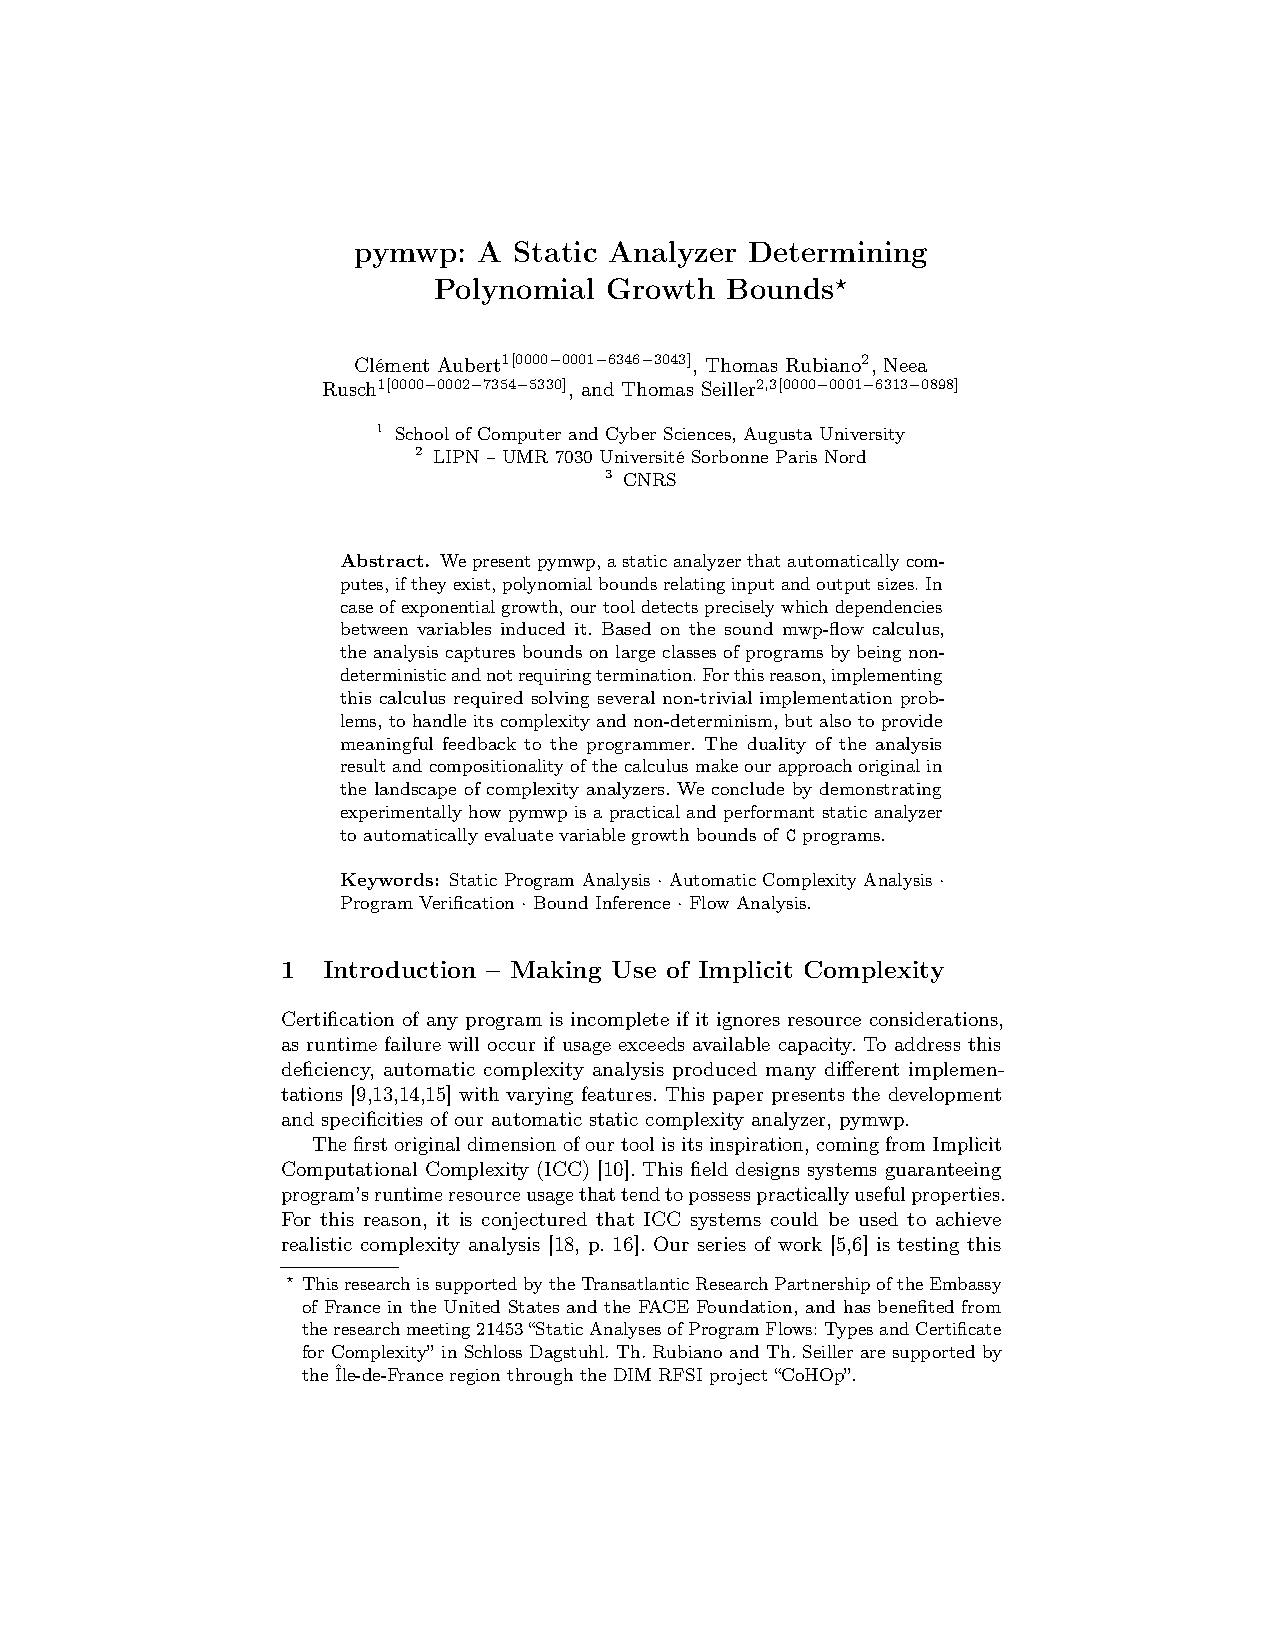
\includepdf[pages={1-}]{pubs/atva/main.pdf}
\linenumbers
